\chapter{Sprint 3 : Gestion des Offres d'Emploi}

\section*{Introduction}

Ce chapitre présente la réalisation du \textbf{sprint 3} de TalentFlow, en lien avec
les user stories US05 et US06 du backlog produit (chapitre~2). S'appuyant sur l'espace
recruteur et les entreprises configurées au sprint~2 (chapitre~4), ce sprint couvre
le cycle de vie des \texttt{OffreEmploi} : création en trois étapes, personnalisation
du formulaire de candidature, publication, génération du \texttt{PublicToken} et
affichage public de l'offre. Nous présentons l'objectif, le backlog, l'analyse des
cas d'utilisation et les interfaces réalisées.

% ============================================================
\section{Objectif du Sprint}
% ============================================================

L'objectif principal de ce sprint est de permettre au tenant de \textbf{créer, configurer
et diffuser} des offres d'emploi :

\begin{itemize}
    \item \textbf{Créer et éditer} des offres (\texttt{OffreEmploi}) via un assistant
    en trois étapes : \textit{Informations}, \textit{Configuration}, \textit{Preview}.

    \item \textbf{Personnaliser le formulaire de candidature} via
    \texttt{FormulaireCandidature} et \texttt{ChampPersonnalise} (types Texte, Nombre,
    Date, ChoixMultiple, Fichier).

    \item \textbf{Publier ou dépublier} une offre (\texttt{EstPublie}) depuis la liste
    ou l'aperçu final.

    \item \textbf{Générer un lien public tokenisé} (\texttt{PublicToken}) et l'associer
    à l'URL \texttt{/public/offres/\{token\}}.

    \item \textbf{Assigner des experts} à une offre (\texttt{AssignationExpert}) et
    proposer une \textbf{page publique} consultable par les candidats et visiteurs.
\end{itemize}

% ============================================================
\section{Analyse du Sprint 3}
% ============================================================

\subsection{Sprint Backlog}

Le tableau~\ref{tab:backlog_s3} présente les user stories réalisées durant ce sprint.

\begin{table}[h]
\centering
\renewcommand{\arraystretch}{1.4}
\begin{tabular}{|c|p{8.5cm}|c|}
\hline
\textbf{ID} & \textbf{User Story} & \textbf{Priorité} \\
\hline
US05 & En tant que tenant, je veux créer et publier une offre d'emploi
(\texttt{OffreEmploi}) afin d'attirer des candidats qualifiés. & Haute \\
\hline
US06 & En tant que tenant, je veux personnaliser le formulaire de candidature
(\texttt{ChampPersonnalise}) et générer un lien public tokenisé (\texttt{PublicToken}). & Haute \\
\hline
US06a & En tant que tenant, je veux lister, filtrer et gérer le statut de publication
de mes offres. & Haute \\
\hline
US06b & En tant que tenant, je veux assigner des experts à une offre pour le suivi
des candidatures. & Haute \\
\hline
US06c & En tant que guest ou candidat, je veux consulter une offre via son lien public
et connaître les conditions de candidature (date limite). & Haute \\
\hline
\end{tabular}
\caption{Sprint Backlog du Sprint 3}
\label{tab:backlog_s3}
\end{table}

\subsection{Diagramme de Cas d'Utilisation — Sprint 3}

\begin{figure}[ht]
    \centering
    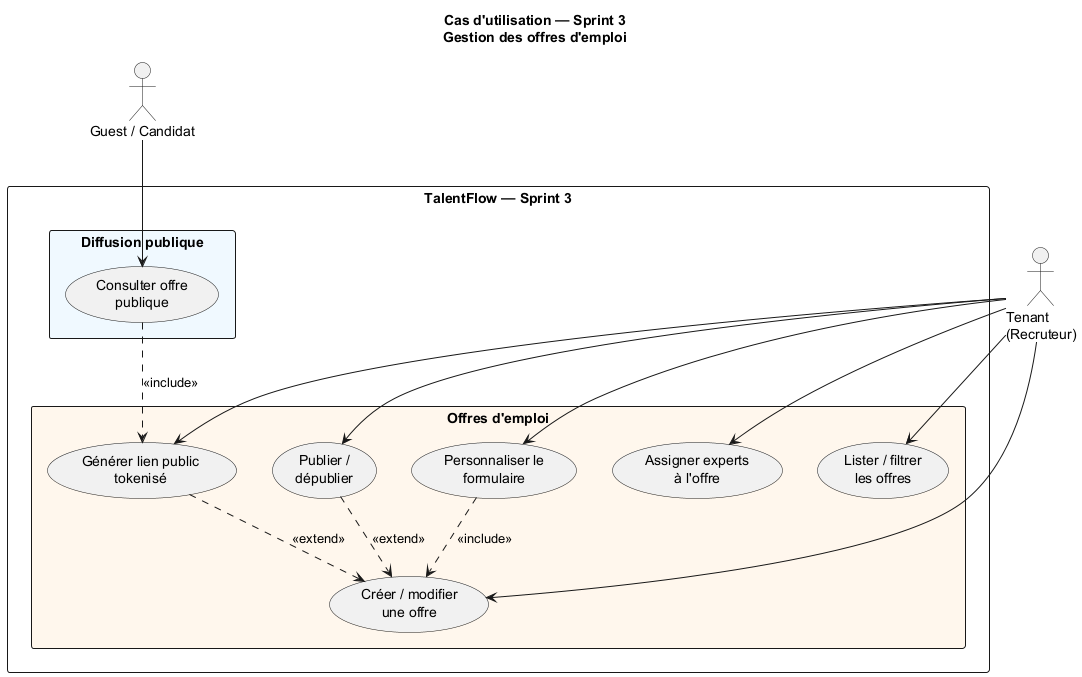
\includegraphics[width=0.95\textwidth]{images/usecase_sprint3.png}
    \caption{Diagramme de cas d'utilisation du Sprint 3}
    \label{fig:uc_sprint3}
\end{figure}

\subsubsection{Description Textuelle des Cas d'Utilisation}

\textbf{Cas d'utilisation : Créer et publier une offre}

\begin{itemize}
    \item \textbf{Acteur principal :} Tenant (recruteur)
    \item \textbf{Précondition :} au moins une \texttt{Entreprise} existe pour le tenant.
    \item \textbf{Scénario nominal :}
    \begin{enumerate}
        \item Étape \textit{Informations} : société, titre, description, lieu, contrat,
        date limite (\texttt{DateLimiteCandidatures}).
        \item Étape \textit{Configuration} : champs personnalisés, lien public, experts.
        \item Étape \textit{Preview} : aperçu candidat, brouillon ou publication
        (\texttt{EstPublie = true}).
    \end{enumerate}
    \item \textbf{Postcondition :} l'offre apparaît dans \textit{Job Offers} et, si
    publiée, est accessible via \texttt{/public/offres/\{token\}}.
\end{itemize}

\textbf{Cas d'utilisation : Consulter une offre publique}

\begin{itemize}
    \item \textbf{Acteur principal :} Guest ou Candidat
    \item \textbf{Précondition :} \texttt{PublicToken} valide, offre publiée.
    \item \textbf{Exception :} si la date limite est dépassée, affichage
    \textit{Candidatures closes}.
    \item \textbf{Postcondition :} consultation de la fiche ; candidature traitée au
    chapitre~6 (sprint~4).
\end{itemize}

% ============================================================
\section{Réalisation}
% ============================================================

\subsection{Liste des Offres d'Emploi}

La page \textit{Job Offers} (\texttt{JobOffers.vue}) regroupe toutes les offres du
tenant avec recherche, filtres par entreprise et par statut (\textit{published} /
\textit{draft}). Chaque ligne affiche le titre, la société, la localisation, le nombre
de candidats, la date de création et des actions (aperçu, édition, publication,
copie du lien public). Le bouton \textit{Create Offer} lance l'assistant en trois étapes.

\begin{figure}[ht]
    \centering
    \includegraphics[width=\textwidth]{images/job_offers_list.jpg}
    \caption{Liste des offres d'emploi du recruteur}
    \label{fig:job_offers_list}
\end{figure}

\subsection{Création d'une Offre — Étape 1 : Informations}

L'assistant (\texttt{CreateJobStep1.vue}) commence par la sélection de l'entreprise,
le titre du poste, la description enrichie (éditeur riche), la localisation, le type
de contrat (CDI, CDD, stage, etc.) et la date limite de candidature.

\begin{figure}[ht]
    \centering
    \includegraphics[width=\textwidth]{images/create_job_step1.jpg}
    \caption{Création d'offre — étape 1 : informations et description}
    \label{fig:create_job_step1}
\end{figure}

\begin{figure}[ht]
    \centering
    \includegraphics[width=\textwidth]{images/create_job_step1b.jpg}
    \caption{Création d'offre — étape 1 (suite) : lieu, contrat et date limite}
    \label{fig:create_job_step1b}
\end{figure}

\subsection{Création d'une Offre — Étape 2 : Configuration}

L'étape \textit{Configuration} (\texttt{CreateJobStep2.vue}) comporte le
\textbf{Form Builder} (\texttt{ChampPersonnalise}) et le panneau \textbf{Job Visibility}
pour activer le \texttt{PublicToken}. L'URL générée peut être copiée ou régénérée.
Des experts peuvent être associés à l'offre depuis cette étape.

\begin{figure}[ht]
    \centering
    \includegraphics[width=\textwidth]{images/create_job_step2.jpg}
    \caption{Création d'offre — étape 2 : formulaire personnalisable}
    \label{fig:create_job_step2}
\end{figure}

\begin{figure}[ht]
    \centering
    \includegraphics[width=0.85\textwidth]{images/create_job_public_link.jpg}
    \caption{Activation du lien public tokenisé (\texttt{PublicToken})}
    \label{fig:create_job_public_link}
\end{figure}

\subsection{Assignation des Experts à une Offre}

La modale \textit{Assign Experts to Job} (\texttt{AssignExpertsModal.vue}) permet
de sélectionner les membres RH participant au recrutement. Les assignations sont
enregistrées dans \texttt{AssignationExpert} (lien expert ↔ offre préparé au sprint~2).

\begin{figure}[ht]
    \centering
    \includegraphics[width=0.85\textwidth]{images/assign_experts_job.jpg}
    \caption{Assignation des experts à une offre d'emploi}
    \label{fig:assign_experts}
\end{figure}

\subsection{Publication et Aperçu (Étape 3)}

L'étape \textit{Preview} (\texttt{CreateJobStep3.vue}) simule le rendu candidat
(\textit{Candidate Preview Mode}), affiche le formulaire personnalisé et les experts
assignés. Le recruteur peut enregistrer un brouillon (\texttt{EstPublie = false}) ou
publier l'offre (\textit{Publish Offer}). L'aperçu est également accessible depuis
la liste via l'icône \textit{Preview}.

\subsection{Affichage Public de l'Offre}

La route \texttt{/public/offres/\{PublicToken\}} (\texttt{PublicJobView.vue}) affiche
l'offre aux visiteurs sans authentification : titre, entreprise, localisation,
description, date limite et type de contrat. Si la date limite est dépassée, le message
\textit{Les candidatures sont closes} s'affiche ; le candidat authentifié pourra
postuler dans le sprint suivant (chapitre~6).

\begin{figure}[ht]
    \centering
    \includegraphics[width=\textwidth]{images/public_job_view.jpg}
    \caption{Page publique d'une offre (lien tokenisé dans la barre d'adresse)}
    \label{fig:public_job_view}
\end{figure}

\subsection{Transition vers le Suivi des Candidatures}

Une fois les offres publiées, le recruteur peut déjà consulter les premières
candidatures depuis \textit{Candidates} (\texttt{Candidates.vue}). Le traitement
complet de l'espace candidat et du pipeline de candidatures est développé au
chapitre~6 (sprint~4).

\begin{figure}[ht]
    \centering
    \includegraphics[width=\textwidth]{images/recruiter_candidates.jpg}
    \caption{Aperçu du suivi des candidatures (transition vers le sprint 4)}
    \label{fig:recruiter_candidates}
\end{figure}

\section*{Conclusion}

Le sprint 3 a complété la chaîne de valeur recruteur : création structurée des
\texttt{OffreEmploi}, formulaires personnalisés, publication, \texttt{PublicToken}
et page publique. Les offres sont désormais diffusables hors de la plateforme tout
en restant rattachées au tenant et à l'\texttt{Entreprise} concernée. Le chapitre
suivant traitera le sprint~4 : espace candidat, dépôt de candidature avec CV sur
Cloudinary et suivi du pipeline.
